\chapter{Logic Gates}
\label{chap:logic-gates}

\chapterintro{Logic gates are physical implementations of Boolean operations. By combining gates, engineers build adders, memory, processors, and complete computers.}

\learningobjectives{
\begin{itemize}
    \item Define a logic gate.
    \item Explain NOT, AND, OR, NAND, NOR, and XOR gates.
    \item Connect Boolean algebra to circuits.
    \item Build simple gate simulations in Python.
\end{itemize}}

\section{From Boolean Algebra to Hardware}

Boolean algebra gives us the rules. Logic gates implement those rules in hardware.

\begin{definition}
A logic gate is a physical or simulated device that accepts one or more binary inputs and produces a binary output.
\end{definition}

\section{The NOT Gate}

A NOT gate has one input and one output. It flips the input.

\begin{center}
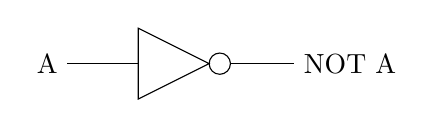
\begin{tikzpicture}[scale=0.9]
\draw (0,0) -- (1,0);
\draw (1,-0.5) -- (1,0.5) -- (2,0) -- cycle;
\draw (2.15,0) circle (0.15);
\draw (2.3,0) -- (3.2,0);
\node[left] at (0,0) {A};
\node[right] at (3.2,0) {NOT A};
\end{tikzpicture}

\end{center}

\section{The AND Gate}

An AND gate outputs \(1\) only when both inputs are \(1\).

\section{The OR Gate}

An OR gate outputs \(1\) when at least one input is \(1\).

\section{The NAND Gate}

A NAND gate is an AND gate followed by a NOT operation. NAND is important because many digital systems can be built entirely from NAND gates.

\section{The XOR Gate}

An XOR gate outputs \(1\) when the inputs are different. XOR is essential for binary addition.

\section{Python Simulation}

\begin{lstlisting}
def nand_gate(a: int, b: int) -> int:
    if a not in (0, 1) or b not in (0, 1):
        raise ValueError("inputs must be 0 or 1")
    return 0 if a == 1 and b == 1 else 1
\end{lstlisting}

\section{Databricks Community Edition Lab}

Create a notebook named \code{volume01\_chapter17\_logic\_gates}. Paste the Python gate functions into the first cell, then create a second cell that generates truth tables for all two-input gates.

\section{Exercises}

\begin{exercise}
Why is the NAND gate sometimes called universal?
\end{exercise}

\begin{solution}
A NAND gate is universal because NOT, AND, and OR can all be constructed using only NAND gates. Since those operations can be combined to produce more complex circuits, NAND alone is sufficient to build digital logic.
\end{solution}

\section{Summary}

Logic gates turn Boolean mathematics into physical computation. The next chapter combines gates to build a half adder.
